\section{Backgrounds}
\label{sect:bkg}
We separate the backgrounds into two categories.  Those with 
``misidentified'' \Tau, i.e., events where a quark or gluon jet has been misidentified
as a \Tau, and those without \Tau misidentifications.  
The misidentified \Tau backgrounds arise mostly from QCD and \wjets events.  The 
other background events are from \ttbar, $Z+$ jets, Higgs boson and diboson events.
Backgrounds with misidentified \Tau are mainly estimated with data-driven methods; the 
remaining backgrounds are taken from Monte Carlo events. The main backgrounds
are discussed here, but the others are very small, so they are  taken from the simulated events.

\subsection{\texorpdfstring{QCD background estimation in the $\tauTau$ channel}{QCD background estimation in the tau-tau channel}}
\label{sect:bkgQCD}
Events from QCD multijet production can enter the signal regions 
if both \Tau arise from misidentified quark or gluon jets
and the rest of the kinematical selections are also satisfied.  
Isolation is an important 
discriminant between misidentified and real \Tau objects. For this purpose, the control regions (CR) are defined using the isolation variables 
for the \Tau pair and \mttwo or \SumMT. To reduce contamination from real \tauTau events, 
in the control regions with at least one loose \Tau object, 
the same-sign (SS) pairs are selected. Residual contributions from real 
\tauTau and \wjets events are subtracted based on Monte Carlo expectations. The control regions and signal region are 
illustrated in Fig.~\ref{fig:ABCDQCD}. 
\begin{figure}[!htb]
\centering
%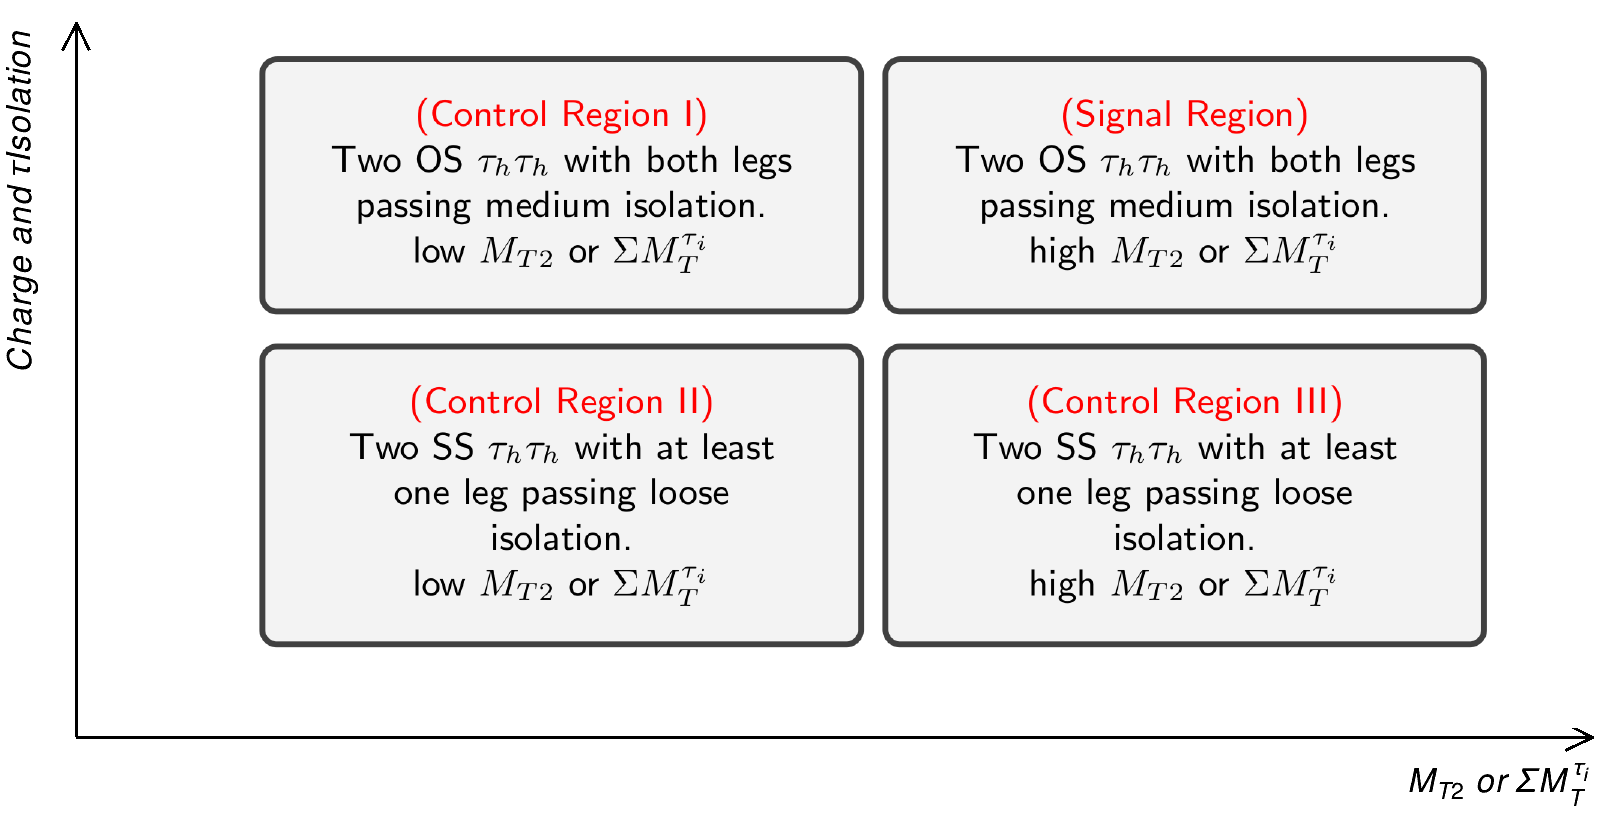
\includegraphics[angle=0,scale=0.28]{Bkg/ABCD.png}
\includegraphics[angle=0,scale=1.15]{Bkg/ABCD.pdf}
\caption{Schematic illustration of four control regions used to estimate the QCD backgrounds. SS and OS stand for same-sign and opposite-sign pairs.}
\label{fig:ABCDQCD}
\end{figure}
In the sample dominated by QCD multijet events (CR1 and CR2), isolations of misidentified \Tau objects verified 
to be uncorrelated with \mttwo or \SumMT.
QCD background in the signal regions are estimated by counting events in the control regions with high \mttwo or \SumMT  
and loosely isolated SS \tauTau (CR3)
and scaling by the transition factor to go from loosely isolated SS to tightly isolated oppsite-sign (OS) 
\tauTau which is evaluated in the low \mttwo or \SumMT (CR1 divided by CR2).

In addition, the requirement on \deltaphi
is removed to improve the statistics of the control regions. 
The final estimate of the background
is taken from the control regions extrapolation with corrections
associated with the same-sign requirement and the efficiency of 
the \deltaphi requirement for QCD events. The latter efficiency is measured in CR1 and CR2 which are dominated by QCD multijet events.
 
Table \ref{4QCDbg} 
\begin{table}[!htb]
\begin{center}
\caption{The estimated QCD multijet background event yields in the \tauTau channel. The first two uncertainties are statistical and systematic uncertainties of the method, the last uncertainty is the extra systematic uncertainty due to correlation assumptions.}
\begin{tabular}{|l|c|}
\hline\hline
 Signal Region      &  Estimation\\
\hline\hline
\tauTau \binone      & 0.13 $\pm$ 0.06(Stat) $\pm$ 0.19(Sys) $\pm$ 0.10 (Fit Unc.) \\
\tauTau \bintwo      & 1.15 $\pm$ 0.39(Stat) $\pm$ 0.70(Sys) $\pm$ 0.25 (Fit Unc.) \\
\hline\hline
\end{tabular}
\label{4QCDbg}
\end{center}
\end{table}
summarizes the estimation of the QCD background contribution in the two signal regions after extrapolation from the control regions and 
correcting for the \deltaphi efficiency.  
The systematic uncertainties are associated with the uncertainty on the validity 
of the assumption that isolation and \mttwo or \SumMT are not correlated and the systematic uncertainties on the residual 
SM backgrounds which  are subtracted based on Monte Carlo expectations. The latter includes both statistical uncertainty of the Monte Carlo 
events and also 28\% systematic uncertainty assigned uniformly to all simulated events.


\subsection{\texorpdfstring{\wjets background estimation in the $\tauTau$ channel}{W+jets background estimation in the tau-tau channel}}
\label{sect:bkgW}
The contribution of the \wjets background in \tauTau channels is taken from simulation where the simulation of this process is validated in a data control sample. 
In different signal regions after the final requirement of \mttwo $>$ 90\GeV or \SumMT $>$ 250\GeV, 
the \wjets Monte Carlo has large statistical uncertainties and the predicted value is not reliable. 
The efficiencies of the final selection requirements, $\epsilon_{\rm M_{T2}}=\frac{N_{\rm M_{T2}>90}}{N_{\rm M_{T2}>40}}$ for  \binone and $\epsilon_{\SumMT}=\frac{N_{\SumMT>250}}{N_{40<\rm M_{T2}<90}}$ for \bintwo, generally referred to as $\epsilon_{FS}$, are evaluated in MC after relaxing some kinematic selections. 
The final estimations can be read as:
\begin{equation}
N_{\rm SR} = N_{\rm Before~Final~Selection} \times \epsilon_{FS}.
\end{equation}
where, $N_{\rm Before~Final~Selection}$ is the number of \wjets events just before applying the final selection 
(\mttwo $>$ 90\GeV for \binone and \SumMT $>$ 250\GeV for \bintwo) and $N_{\rm SR}$ is the final estimation of \wjets events in the signal region.


The $\epsilon_{FS}$ is first evaluated in a \wjets sample with a pair of opposite-charge \Tau where the \Tau candidates are selected similar to those in signal region. 
Additional signal selection requirements, such as \deltaphi or lepton veto, are applied one by one such that two orthogonal subsamples (passing and failing) are obtained. The $\epsilon_{FS}$ quantity is calculated in all subsamples. The values are found to be compatible within the statistical uncertainties; their weighted average is taken as the final estimate for $\epsilon_{FS}$ with weights corresponding to the size of the simulated sample at each step. %The uncertainty on the \Tau energy scale introduces the largest variation on $\epsilon_{FS}$. This variation is considered as a systematic uncertainty on the estimated efficiency.
The uncertainty on $\epsilon_{FS}$  also takes into account the effect of the \Tau energy scale.

The \wjets MC is validated in data using a same-sign \muTau control sample, where both the normalization and $\epsilon_{FS}$ are checked. 
The normalization is found to be compatible between data and simulation, within uncertainties. For $\epsilon_{FS}$, 
to take into account the difference between the data and MC values, the MC prediction in each
of the two search regions is corrected by the ratio of the two values and its uncertainty is also
taken into account. This part of the systematic uncertainty is referred to as ``sys. shape''"

Table \ref{tbl:Wbkg} summarizes the results of  the method for different signal regions of the \tauTau channel.
\begin{table}[!htb]
\begin{center}
\caption{The \wjets estimation results in both search regions. The systematics (sys.) comes from the maximum
variation of the estimation found  from varying the \Tau energy scale within its uncertainty.
 The ``sys. shape'' takes into account the difference between the shape of the search variable distribution in data and Monte Carlo.}
\begin{tabular}{|l|c|}
\hline\hline
Signal Region & \wjets Estimation Results\\
\hline
\tauTau \binone & 0.72 $\pm$ 0.11 (stat.) $\pm$ 0.11 (sys.) $\pm$ 0.56 (sys. shape)\\
\tauTau \bintwo & 2.58 $\pm$ 0.35 (stat.) $\pm$ 1.04 (sys.) $\pm$ 0.69 (sys. shape)\\
\hline\hline
\end{tabular}
\label{tbl:Wbkg}
\end{center}
\end{table}

\subsection{Drell-Yan background estimation}
The Drell-Yan (DY) background yield is obtained from Monte Carlo simulation. The Monte Carlo sample is inclusive for leptons and 
includes decay to different lepton pairs ($ee$, $\mu\mu$ and $\tau\tau$). It is validated that the contribution from $ee$ and $\mu\mu$
is very small, but for the \leptonTau channels the contribution from these events which have a real lepton and a misidentified \Tau 
is evaluated in the next section, when \wjets contribution is estimated.
The simulation is validated in a \muTau control region obtained by removing the \deltaphi
requirement and by inverting the \Z boson veto and also (\mttwo $<$ 20\GeV,  40 $<$ \tauMT $<$ 100\GeV).  
The distribution of invariant mass of ($\mu, \Tau$) system for data and Monte Carlo events have a good agreement.
The transverse momentum of the \Z boson system, which is correlated with 
\mttwo, is also well reproduced in simulation. Table \ref{tbl:DYbkg}
\begin{table}[!htb]
\begin{center}
\caption{DY background yield expected in four signal regions. 
%The first uncertainty is statistical and the second is systematic. The systematic uncertainties assigned to the central values are discussed in Section \ref{sect:sys}.}
Only the statistical uncertainties are reported.}
\begin{tabular}{|l|c|}
\hline\hline
Signal Region      &  DY Estimation\\
\hline\hline
\eTau              & 0.20  $\pm$  0.13\\\hline%  $\pm$ 0.05 \\\hline
\muTau             & 0.26  $\pm$  0.13\\\hline%  $\pm$ 0.07 \\\hline
\tauTau \binone    & 0.56  $\pm$  0.07\\\hline%  $\pm$ 0.16 \\\hline
\tauTau \bintwo    & 0.81  $\pm$  0.56\\\hline%  $\pm$ 0.23 \\
\hline\hline
\end{tabular}
\label{tbl:DYbkg}
\end{center}
\end{table}
summarizes the DY contribution in different signal regions. 
For $\ell\Tau$ channels, only the contributions from the real lepton + \Tau are reported. 
A separate method is developed to estimate the misidentified contamination in these channels.


\subsection{\texorpdfstring{Misidentified \Tau in the $\ell\Tau$ channels}{Misidentified tau in the lepton-tau channels}}
\label{sect:bkgFake}
This contribution is estimated using a fake rate method.
When the loose signal selection is applied, the number of loose $\hadtau$ ($N_{\rm Loose}$) is:

\begin{equation}
N_{\rm Loose} = N_{\rm Real} + N_{\rm Fake}
\end{equation}
where $N_{\rm Real}$ is the number of real $\hadtau$ and $N_{\rm Fake}$ is the number of misidentified 
$\hadtau$. If the selection is tightened, the number of tight $\hadtau$ ($N_{\rm Tight}$) is

\begin{equation}
 N_{\rm Tight} = r_{\rm Real}.N_{\rm Real} + r_{\rm Fake}.N_{\rm Fake}
\end{equation} 
where $r_{\rm Real}$ ($r_{\rm Fake}$) is the real (fake) rate, the probability that a loosely selected real (misidentified) $\hadtau$ passes the  tight  selection. 
The loose category ($N_{\rm Loose}$) can be divided to two parts, 
tight ($N_{\rm Tight}$) and non-tight ($N_{\rm NTight}$), so one can obtain the following expression by eliminating $N_{\rm Real}$:

\begin{equation}
   N_{\rm Fake}.(r_{\rm Fake}-r_{\rm Real}) = ((1 - r_{\rm Real}).N_{\rm Loose}  - N_{\rm NTight})
\end{equation}
$r_{\rm Fake}$.$N_{\rm Fake}$ is the contamination of misidentified $\hadtau$ to the signal region. 

The fake rate ($r_{\rm Fake}$) is measured as the ratio of tightly selected $\hadtau$ to loosely 
selected $\hadtau$ in a sample which is dominated by misidentified $\hadtau$. This is done in a sample of same-sign $\ell\Tau$ selected 
with the same requirements as the opposite-sign $\ell\Tau$
selection for the signal.
The fake rate is corrected by the difference found in MC between the 
same-sign and opposite-sign fake rates which is 1.144 $\pm$ 0.019.
The final value of the fake rate is $r_{\rm Fake}$ = 0.51 $\pm$ 0.01. 
As a cross check, the fake rate was also measured in an opposite sign region with a reversed
\MPT requirement, i.e., \MPT $<$ 30\GeV.
A consistent value is measured for the fake rate.  
The real rate ($r_{\rm Real}$) is measured in Monte Carlo DY events, and it is found to 
be $r_{\rm Real}$ = 0.766 $\pm$ 0.003 independent of \mttwo. 
For both fake rate and real rate, 5\% relative systematic uncertainty is assigned to the central values, although 
by varying the selections, no significant change in the values is seen.

To validate the fake rate method, it is applied to a \wjets Monte Carlo event sample. 
It correctly
predicts the number of $\ell\Tau$ background events in this sample, within the 
uncertainties.
These include statistical uncertainties due to the number of events in the 
sidebands (loosely selected \Tau) as well as 
systematic uncertainties.
The uncertainties on the %variation of the method to estimate the 
fake rate and the real rate %and their statistical uncertainties 
are negligible compared to the statistical uncertainties associated with 
the sidebands. 

The estimates of the misidentified \Tau contamination in the two $\ell\Tau$ 
channels are summarized in Table~\ref{Tab.FakeEstimation}. 
\begin{table}[!htb]
\begin{center}
\caption{Estimation of the misidentified \Tau contribution in the signal region of the $\ell\Tau$ channels. The total systematic is the
quadrature sum of the fractional systematics. All uncertainties are relative.
$r_{\rm Fake}$ ($r_{\rm Real}$) is shorthand for fake (real) rate.}
\begin{tabular}{|l|c|c|c|c|c|}
\hline
\hline
Channel    & Total Fake & rel. Stat &  $r_{\rm Fake}$ Sys & $r_{\rm Real}$  Sys & Total Unc. \\\hline\hline
\muTau     &   6.83     &  56\%     &  16\%    & 3\%  & 59\%  \\
\eTau      &   2.73     &  101\%    &  16\%    & 5\%  & 102\%  \\
\hline
\hline
\end{tabular}
\label{Tab.FakeEstimation}
\end{center}
\end{table}
The relative statistic and systematic uncertainties are reported separately. 
Since the fake rate and real rate are in common between the two 
$\ell\Tau$ channels, the total systematic uncertainties are considered 
fully correlated between the two channels.
